%!TEX encoding = UTF-8 Unicode
\documentclass[12pt]{article} 
\usepackage[left=0.75in,top=20mm,right=0.75in,bottom=0.3in]{geometry} % Document margins
\usepackage{CJK}
\usepackage{graphicx}
\usepackage{mathtools}
\usepackage{mathrsfs}
\usepackage{amssymb}
\usepackage{hyperref}
\usepackage{sidecap}
\usepackage{makecell}
\usepackage{fancyhdr}

\fancypagestyle{title}{
  \setlength{\headheight}{15pt}
  \fancyhf{}
  \renewcommand{\headrulewidth}{0pt}
  \renewcommand{\footrulewidth}{0pt}
  \fancyhead[R]{Parallel Programming 2015}
}

\pagestyle{title}

\makeatletter
\renewenvironment{itemize}
{\list{$\bullet$}{\leftmargin\z@ \labelwidth\z@ \itemindent-\leftmargin
\let\makelabel\descriptionlabel}}
{\endlist}
\makeatother

\begin{CJK}{UTF8}{bsmi}
\title{\textbf{ Homework 3 / Mandelbrot set }}
\author{\textbf{李豪韋 (HW-Lee) ID 103061527}}
\date{}

\begin{document}
\vspace*{-60pt}
{\let\newpage\relax\maketitle}
\thispagestyle{title}

\section*{Overview}
\vspace{-20pt}
\noindent\makebox[\linewidth]{\rule{\textwidth}{0.4pt}}
\vspace{5pt}

Assumed that there is an infinite sequence $Z(c) = \{z_n|n \in \mathbb{N}\}$ that can be generated by a complex number $c$ with a recursive mapping $z_{n+1} = z_n^2 + c$ where $z_1 = c$, the Mandelbrot set is a set of complex numbers such that all elements in $Z(c)$ do not diverge to infinity. Mathematically, the Mandelbrot set can be defined as $\mathbb{M} = \{c|\displaystyle\lim_{n \to \infty}\|z_n(c)\| < \infty , c \in \mathbb{C}\}$, and it can be derived into the further form that we can obtain it more easily:
\begin{center}
    $\mathbb{M} = \{c|\displaystyle\lim_{n \to \infty}\|z_n(c)\| < 2 , c \in \mathbb{C}\}$
\end{center}

To implement a program that computes the Mandelbrot set in an numerical way, the complex space must be bounded by a specific rectangular and the sampling resolution must be designated. Moreover, we cannot check if the sequence remains a small enough norm with infinity, the maximal number of iterations must be defined as well. In this way, the program will be able to obtain the Mandelbrot set by sampling points in the region and determining if the point belongs to the Mandelbrot set if $\|z(c)_{MAX_ITER}\| < 2$. For the convenience of discussing it in more detailed way, each point will be coloured with its iterations into gray-scaled. After all, the output image looks like below:

\begin{center}
    \begin{SCfigure}[][ht]
        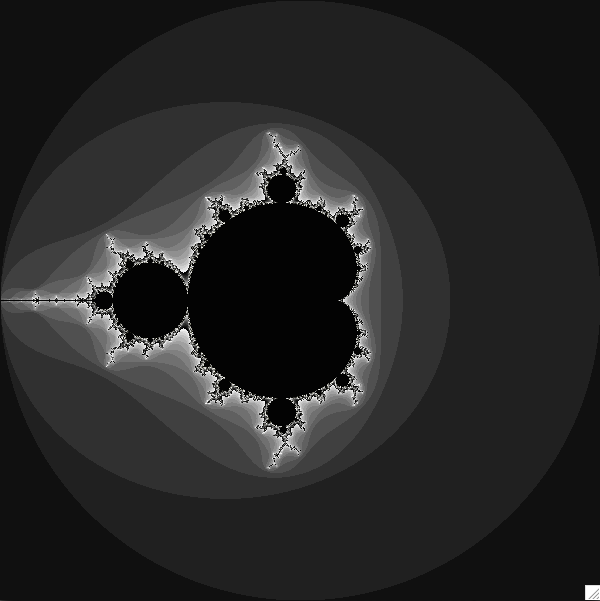
\includegraphics[scale=.5]{./coloring_ta.png}
        \caption{An example showing the Mandelbrot set where the points are ranged from $(-2, -2)$ to $(2, 2)$. Note that the brightness does not directly refer to the magnitude, the raw iterations are processed with modulo function to pronounce the difference between each pair of adjacent region. Therefore, we can observe the 'transition' between adjacent regions easily. However, I think this coloring method is not such good and the coloring methods I use will be discussed in the following section.}
    \end{SCfigure}
\end{center}

\newpage

Obviously, it is important to decide the strategy separating jobs. Because the number of iterations of the point seems to be subjected to the distance from the origin rather than the position, simply deviding the data into a couple of equally large subsets might induce a bad speedup performance due to the unbalanced loads among workers. Therefore, the project is aimed at making us get familiar with APIs and analyze/fine tune a better scheduling strategy.

\section*{Implementation}
\vspace{-20pt}
\noindent\makebox[\linewidth]{\rule{\textwidth}{0.4pt}}
\vspace{5pt}

In the project, the program is implemented with three different APIs, MPI/OpenMP/Hybrid, and two different scheduling strategies, static/dynamic.

\begin{itemize}
    \item Static scheduling: each worker processes same number of columns.
    \vspace{-.5cm}
    \begin{SCfigure}[][ht]
        \hspace{-1cm}
        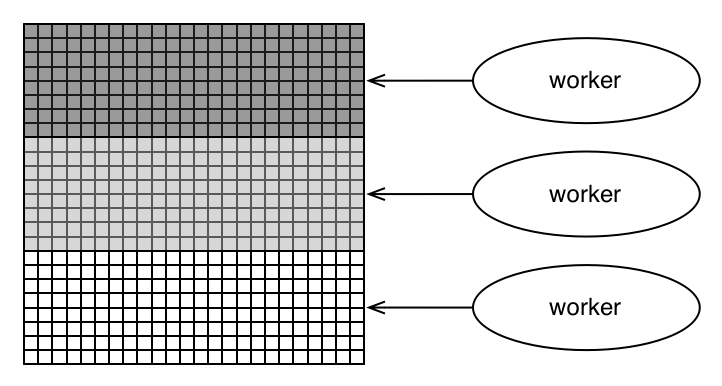
\includegraphics[scale=.5]{./flow_chart_static.png}
        \hspace{-.5cm}
        \vspace{-2cm}
        \caption{Static scheduling: the whole data will be equally separated into several pieces and each work processes its own piece.}
    \end{SCfigure}
    \vspace{1cm}
    \item Dynamic scheduling: each column is assigned dynamically to the worker which completes its task.
    \vspace{-.5cm}
    \begin{SCfigure}[][ht]
        \hspace{-1cm}
        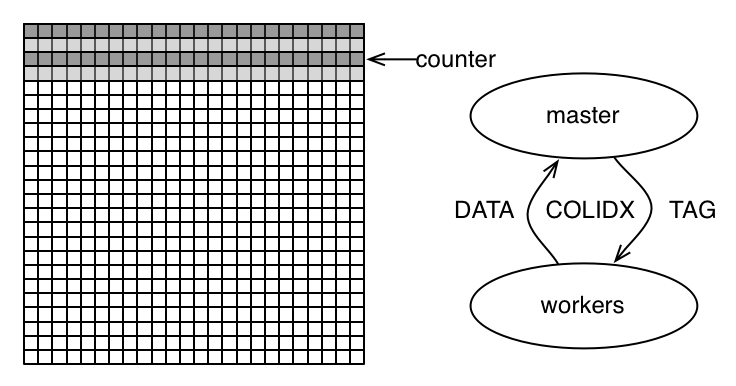
\includegraphics[scale=.5]{./flow_chart_dynamic.png}
        \hspace{-.5cm}
        \vspace{-.5cm}
        \caption{Dynamic scheduling: Only a small batch of columns are assigned to specific workers at the begining, and there is a master that monitors if each worker completes its job and then sends the next job and increments the counter until there is no job remains in the queue. This way provides a more flexible assigning strategy that keeps all workers work during the program.}
    \end{SCfigure}
\end{itemize}

In Hybrid implementations, they follow the same jobs partition strategies as MPI implementations do, and OpenMP is applied when processing a column by dynamically assigning each point in the column to threads.

\newpage

\vspace{-2cm}
\section*{Results}
\vspace{-20pt}
\noindent\makebox[\linewidth]{\rule{\textwidth}{0.4pt}}

\begin{itemize}
    \item Strong Scabilily
    \begin{SCfigure}[][ht]
        \hspace{-1cm}
        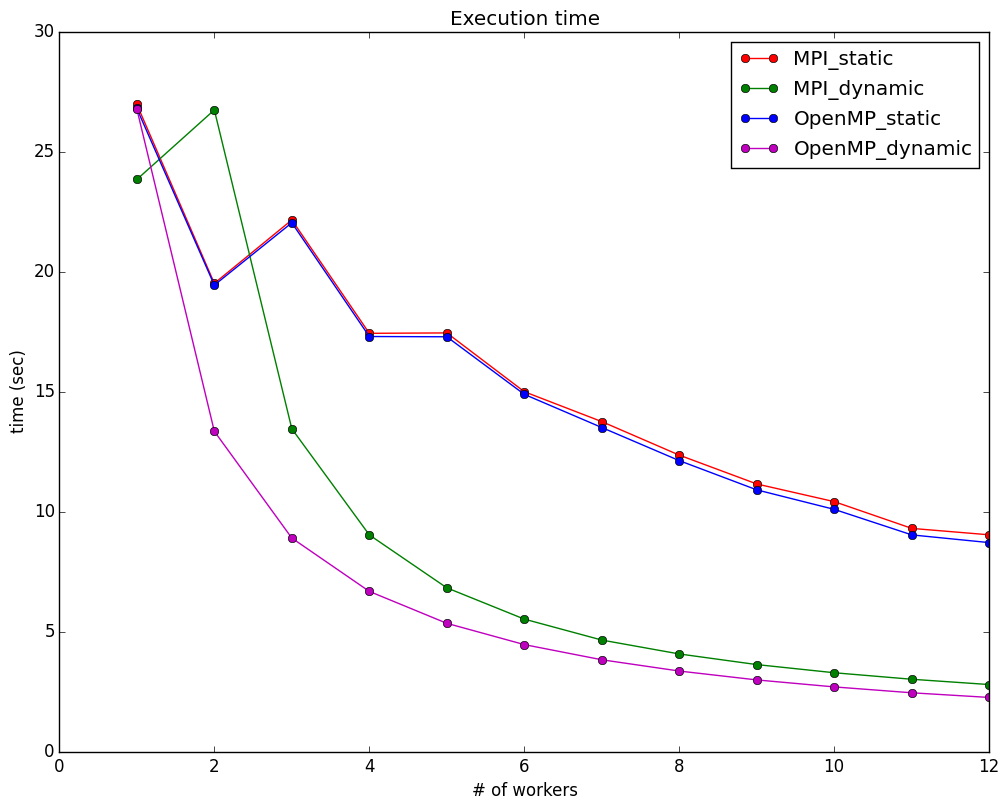
\includegraphics[scale=.5]{./exec.png}
        \vspace{-3cm}
        \caption{Strong scability: static implementations show roughly linear decay and dynamic ones show roughly reverse-propotional decay as the number of workers increases}
        \vspace{2.5cm}
    \end{SCfigure}
    \item Weak Scability
    \begin{SCfigure}[][ht]
        \hspace{-1cm}
        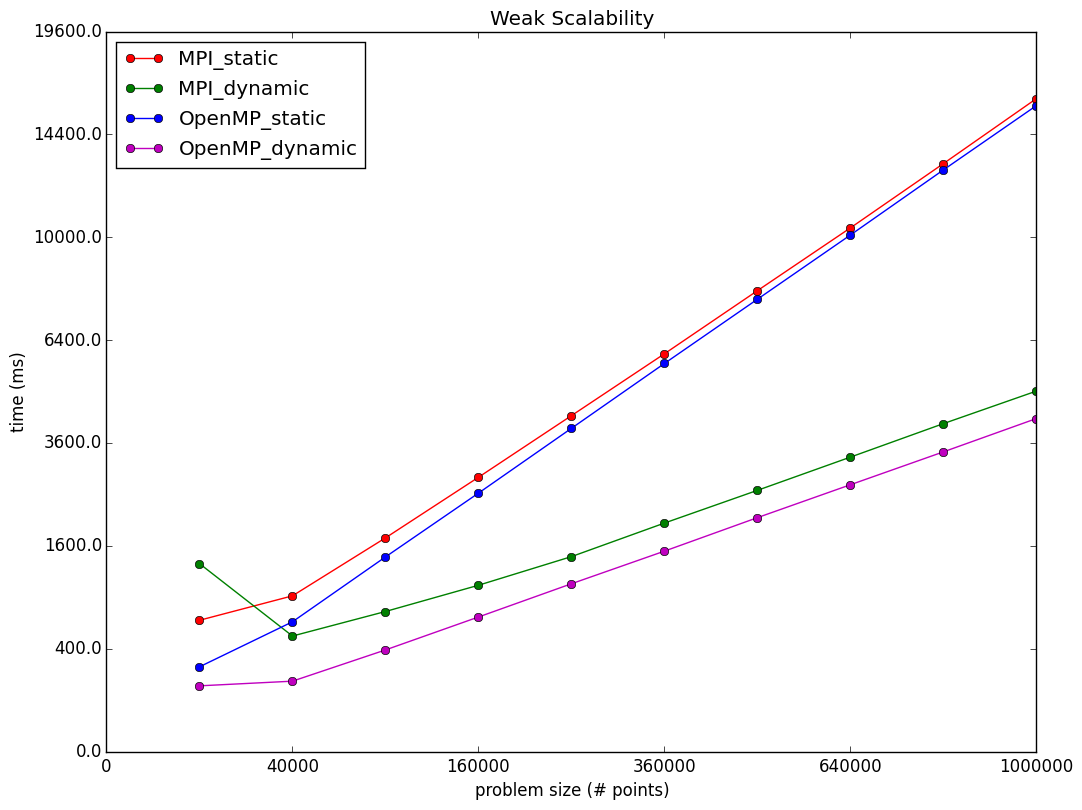
\includegraphics[scale=.5]{./problemsize.png}
        \vspace{-.5cm}
        \caption{Weak scability: all implementations show roughly linear rise as the number of processed points increases}
        \vspace{-1cm}
    \end{SCfigure}

    \newpage

    \item Cost of each worker
    \begin{figure}[ht]
        \hspace{-1cm}
        \begin{minipage}{.48\textwidth}
            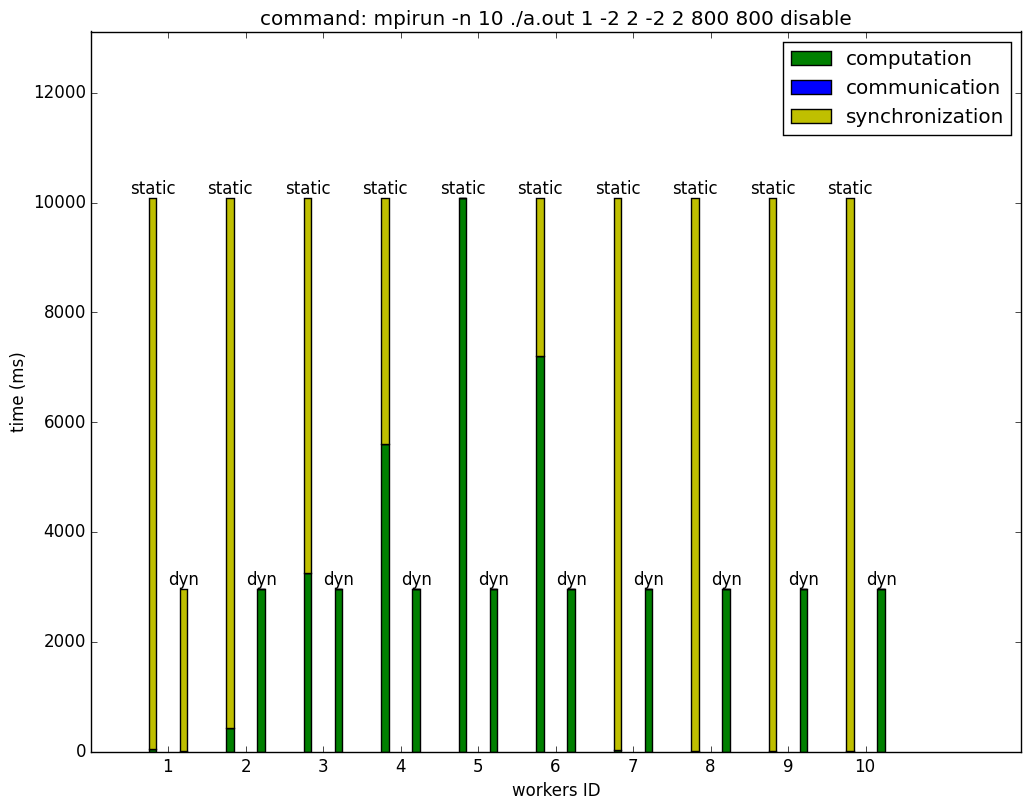
\includegraphics[scale=.35]{./threads_load_MPI.png}
        \end{minipage}
        \hspace{1cm}
        \begin{minipage}{.48\textwidth}
            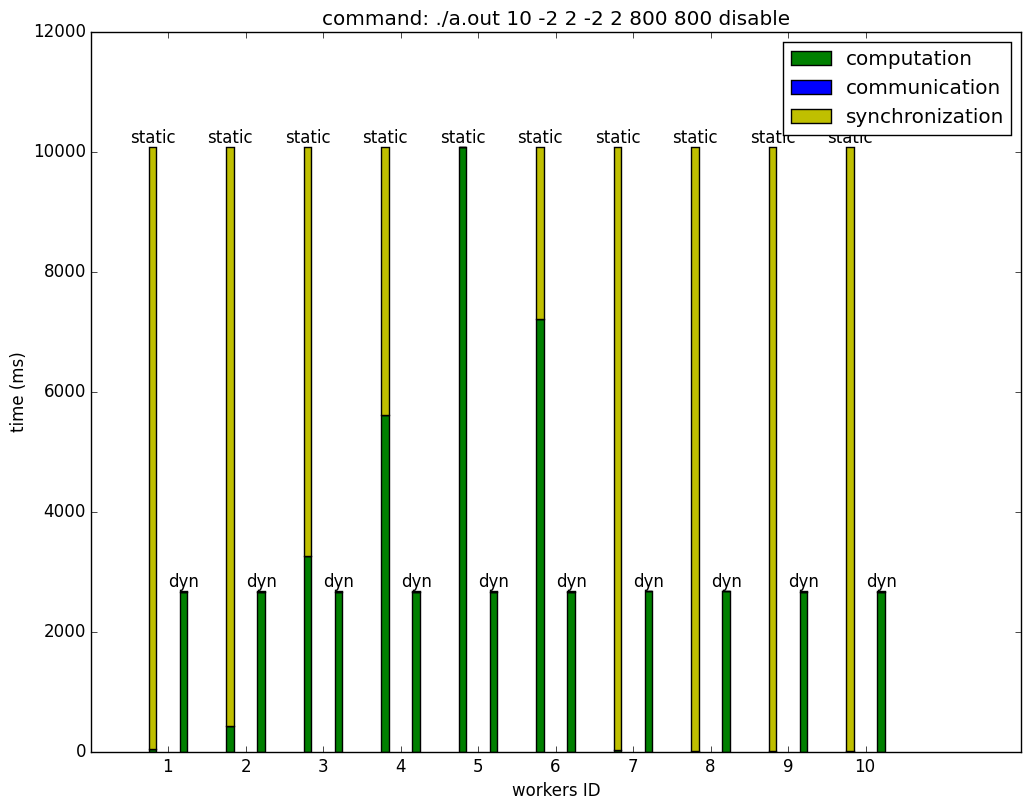
\includegraphics[scale=.35]{./threads_load_OpenMP.png}
        \end{minipage}
    \end{figure}

    \vspace{-1cm}
    \begin{SCfigure}[][ht]
        \hspace{-1cm}
        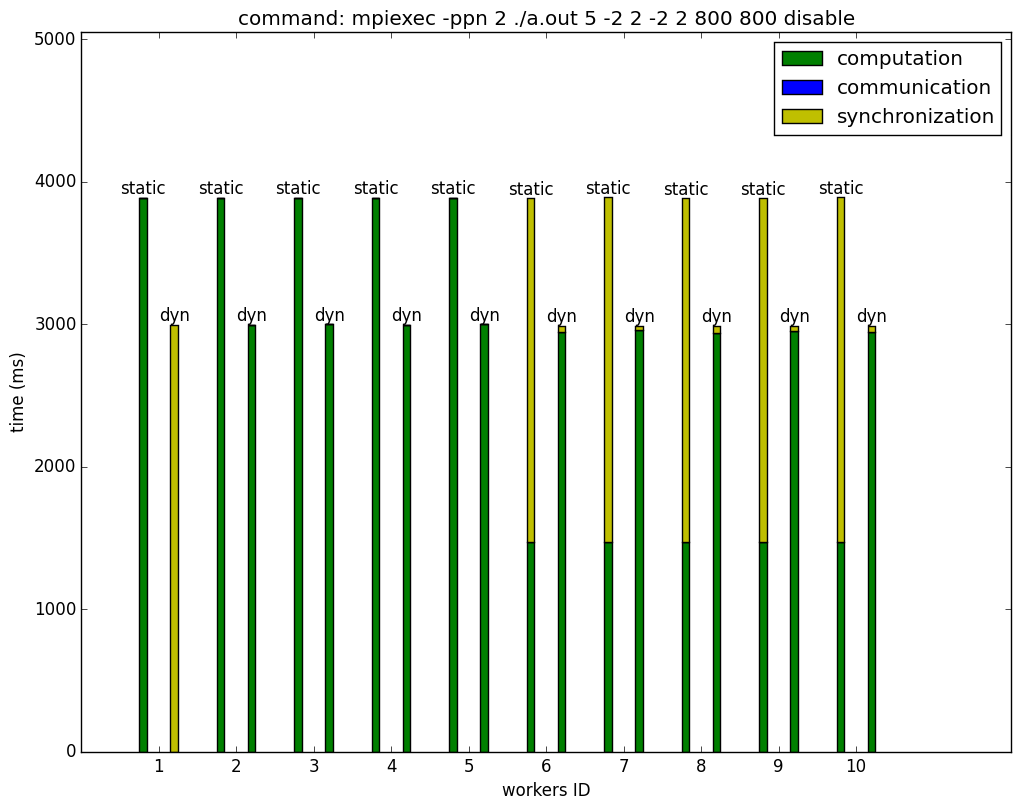
\includegraphics[scale=.35]{./threads_load_Hybrid.png}
        \hspace{1cm}
        \vspace{-.5cm}
        \caption{Loads of each worker: \hspace{\textwidth}MPI(left-upper), OpenMP(right-upper), and Hybrid(left-lower). Execution time is highly dominated by the worker who processes the toughest part of data in static implementations, while it is equally distributed to workers such that the synchronization is very low in dynamic implementations. Note that worker0 always waits for others in both MPI and Hybrid implementation because the worker is assigned to be the master that manages scheduling and handles the parallel jobs.}
    \end{SCfigure}

    \vspace{-.5cm}
    \item Speedup
    \begin{SCfigure}[][ht]
        \hspace{-1cm}
        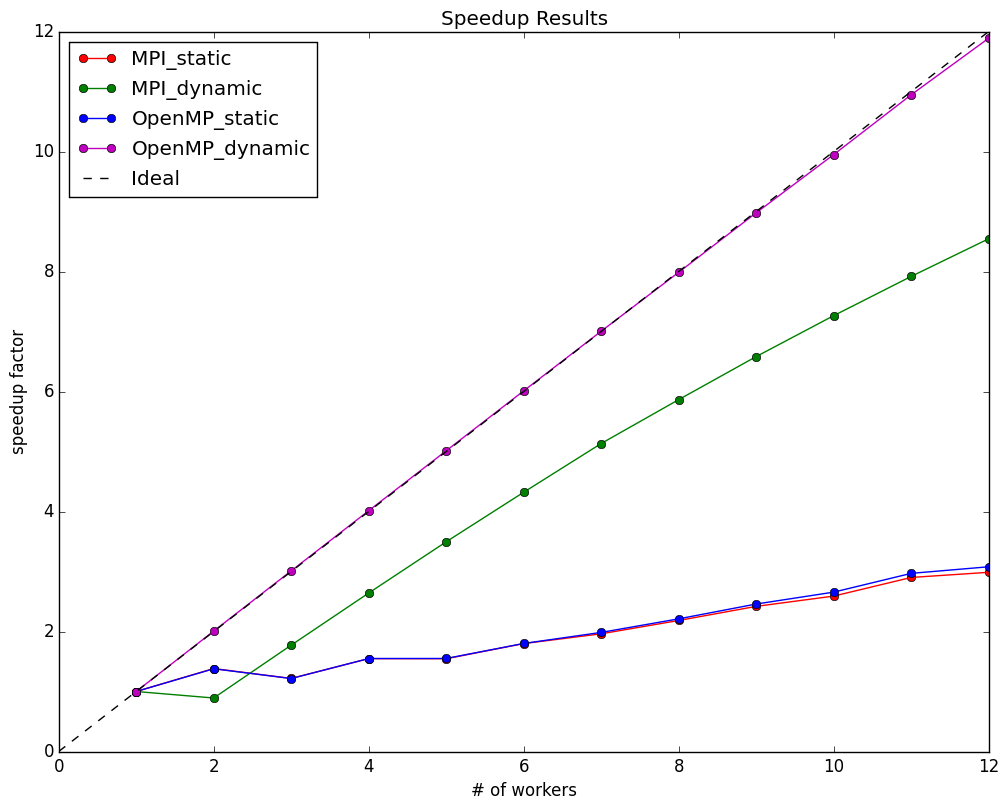
\includegraphics[scale=.45]{./speedup.png}
        \vspace{-.5cm}
        \caption{Speedup factors}
        \vspace{-5cm}
    \end{SCfigure}
\end{itemize}

\newpage

\section*{Analysis \& Discussion}
\vspace{-20pt}
\noindent\makebox[\linewidth]{\rule{\textwidth}{0.4pt}}

\begin{itemize}
    \vspace{-10pt}
    \item Computation complexity
    \begin{flushleft}
        Assumed that there are $N_{pt}$ points need to be computed by $N_{wks}$ workers with a maximal number of iterations $N_{mxit}$, and then the complexity can be obtained as below:
    \end{flushleft}
    \begin{center}
        \begin{tabular}{|c|c|c|c|c|}
            \hline
            \diaghead{\theadfont Diag ColumnmnHead II}{Implementation}{Type} & Comm. & Comp. & Overall & Prop. to \\
            \hline
            MPI & $O\Big(N_{pt}\Big)$ & $O\Big(\frac{N_{pt}N_{mxit}}{N_{wks}-1}\Big)$ & $O\Big(\frac{N_{pt}N_{mxit}}{N_{wks}-1}\Big)$ & $\frac{1}{N_{wks}-1}$ \\
            \hline
            OpenMP & N/A & $O\Big(\frac{N_{pt}N_{mxit}}{N_{wks}}\Big)$ & $O\Big(\frac{N_{pt}N_{mxit}}{N_{wks}}\Big)$ & $\frac{1}{N_{wks}}$ \\
            \hline
            Hybrid & $O\Big(N_{pt}\Big)$ & $O\Big(\frac{N_{pt}N_{mxit}}{N_{wks}-1}\Big)$ & $O\Big(\frac{N_{pt}N_{mxit}}{N_{wks}-1}\Big)$ & $\frac{1}{N_{wks}-1}$ \\
            \hline
        \end{tabular}
    \end{center}
    \begin{flushleft}
        In MPI/Hybrid implementations, communication only used for gathering computed results and the complexity, therefore, can be estimated as $O(N_{pt})$, which means it is propotional to the problem size. In fact, it should be $O(N_{pt} + \sqrt{N_{pt}})$ in dynamic implemenations because the master must send $\sqrt{N_{pt}}$ indices of colunms to slaves during the operations. However, it is much smaller than computation loadings so communication consumptions can be ignored. In computation stage, the complexity should be propotional to $N_{pt}$, $N_{mxit}$, and $\frac{1}{N_{wks}-1}$ (because one worker must be the master managing working process dynamically) then it is noted as $O(\frac{N_{pt}N_{mxit}}{N_{wks}-1})$. After all, the observed results fit the expectation shown above then I can conclude that the implemenations work well and reasonably.
    \end{flushleft}

    \item Speedup results
    \begin{flushleft}
        According to Figure 7, it shows dynamic implementations are superior to static ones. Both dynamic implementations yield good results: which grow linearly as the number of workers increases, and the performance of dynamic MPI saturates gradually at high number of workers, the fact might be caused by communication. \\
        In fact, all implementations show the results decaying linearly as the number of workers increases. However, execution time of static implementations is always dominated by the toughest regions which require lots of iterations to check if each point belongs to the Mandelbrot set. Therefore, the efficiency of parallelizing is not significant.
    \end{flushleft}

    \newpage

    \item Work scheduling
    \begin{flushleft}
        The figures shown below illustrate how the works have been partitioned, and the numbers at the end of labels refer to the number of columns that are assigned to the corresponded worker. In such visualization, the fact that equally separating tasks into several parts is not a good strategy because the loadings of workers are not balanced. To pronounce the correctness of this conclusion, the computation time is visualized with log-scale so that how unbalanced the works are can be easily observed.
    \end{flushleft}
    \begin{figure}[ht]
        \hspace{-2cm}
        \begin{minipage}{.48\textwidth}
            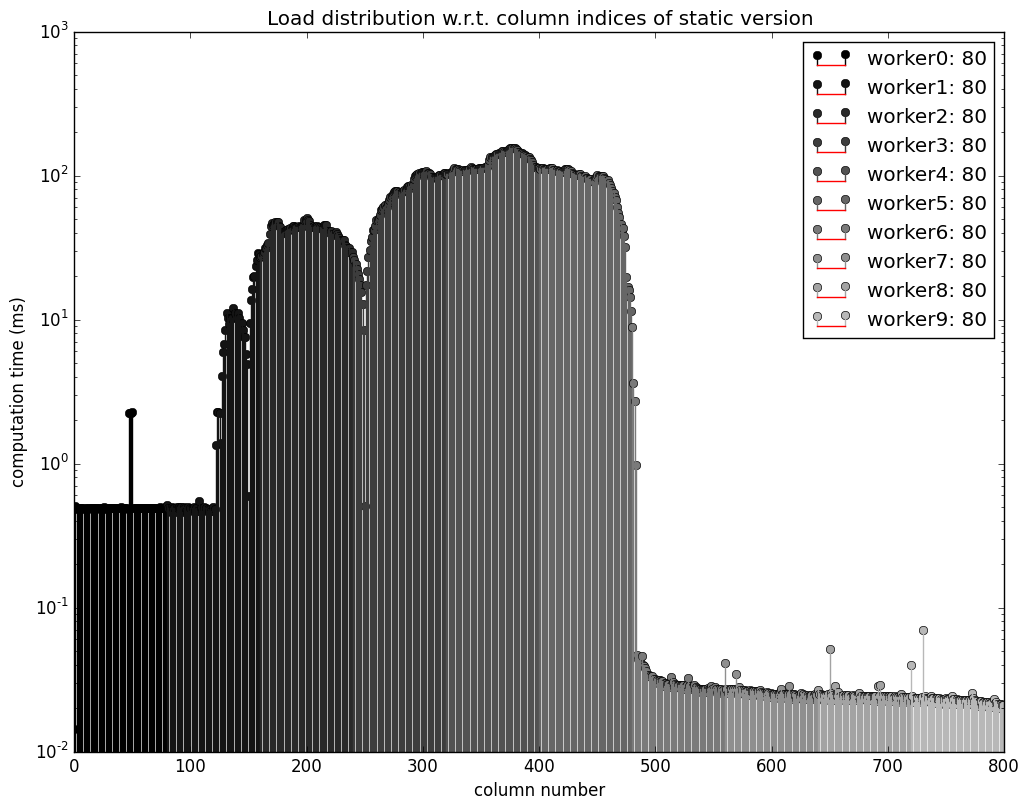
\includegraphics[scale=.4]{./load_dist_static.png}
        \end{minipage}
        \hspace{2cm}
        \begin{minipage}{.48\textwidth}
            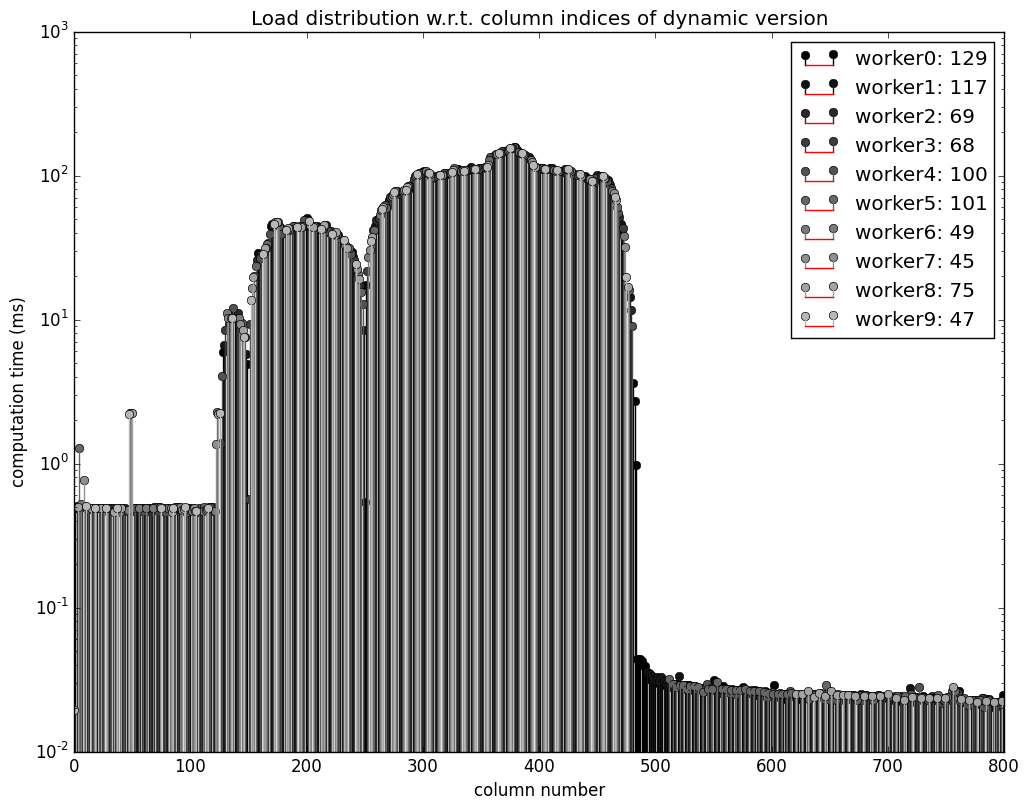
\includegraphics[scale=.4]{./load_dist_dynamic.png}
        \end{minipage}
    \end{figure}

    \item Performance with various resource configurations
    \begin{SCfigure}[][ht]
        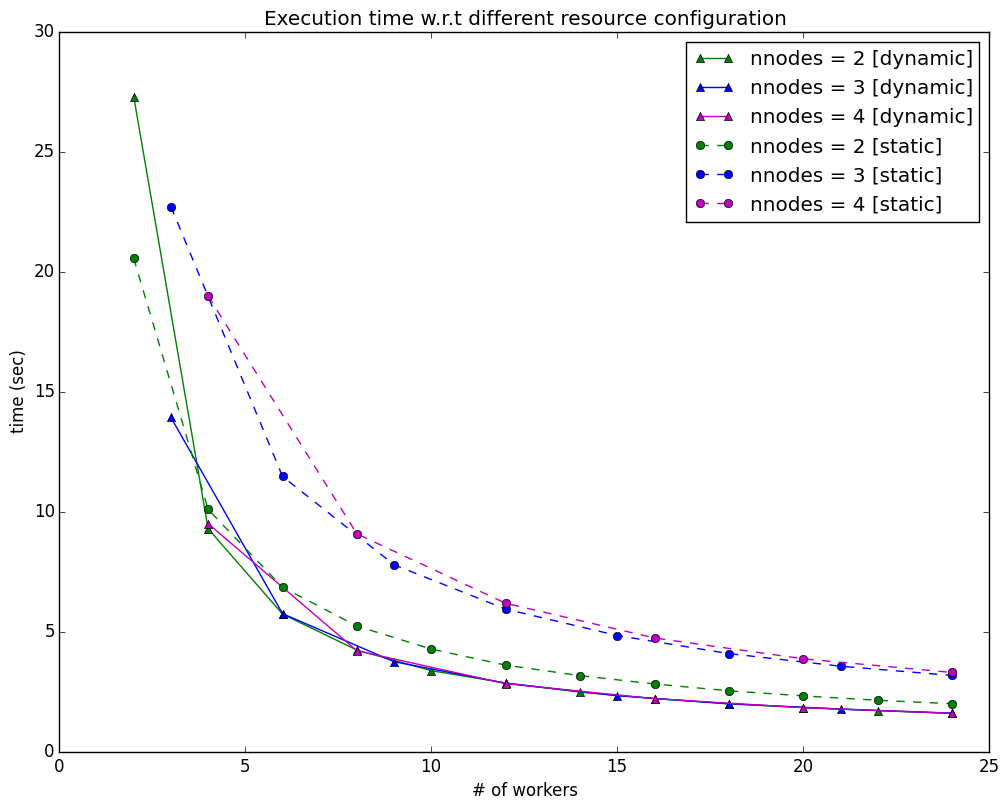
\includegraphics[scale=.5]{./res_dist_exec.png}
        \vspace{-.5cm}
        \caption{Execution time with different number of nodes/ppn: the results show that there is little difference between configurations when applying dynamic scheduling, while applying static scheduling with two nodes seems to be a better choice.}
    \end{SCfigure}

    \item Coloring
    \begin{flushleft}
        In addition to all works mentioned above which are related to performance concerns, the way checking if the program works accurately is also important. Therefore, it might be a good solution to display a 2-D diagram where each pixel refers to iterations at that position because the results can be checked visually/intuitively. The mapping function mapped from integers to gray scales suggested originally is $f(x) = (x \mod 256) / 255.0$, this function, however, cannot acctually illustrate the real magnitude, i.e. $f(x) \ngtr f(y)$, $\forall x > y$. As a result, I decide to use sigmoid function $\phi(x) = \frac{1}{1 + \exp(-x)}$ and propose a monotonic function $g(x) = 2 \times \phi(\log(x)) - 1$, $g(x) \in [0, \, 1]$. \\ The visual results have been shown below:
    \end{flushleft}
    \begin{figure}[ht]
        \begin{minipage}{.48\textwidth}
            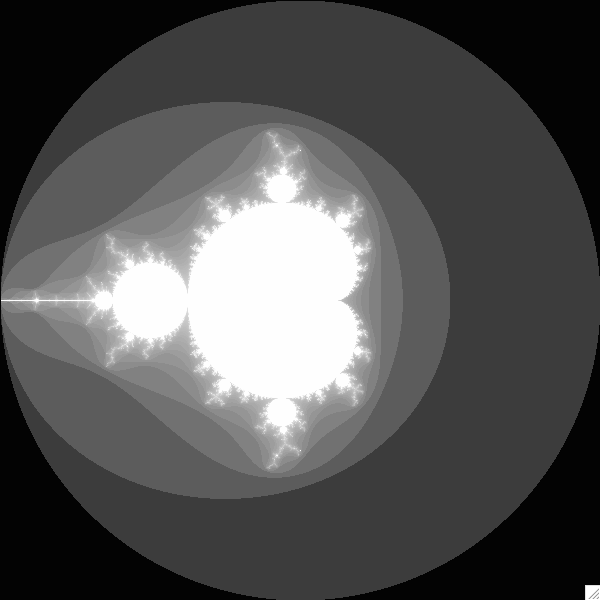
\includegraphics[scale=.4]{./coloring_hw.png}
            \caption{Visual result (8-bit)}
        \end{minipage}
        \begin{minipage}{.48\textwidth}
            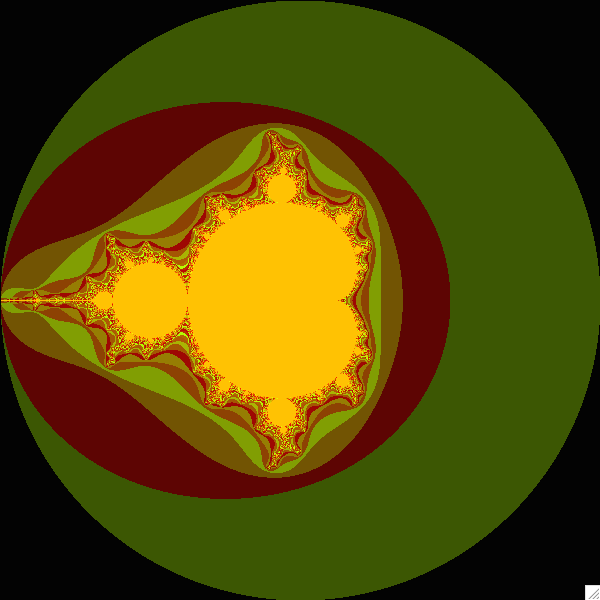
\includegraphics[scale=.4]{./coloring_16bit.png}
            \caption{Visual result (16-bit)}
        \end{minipage}
    \end{figure}
\end{itemize}

This project provides an practice to experience advantages and disadvantages of MPI/OpenMP relatively, and to make good use of both models and optimize the algorithm we want to implement.

\begin{itemize}
    \item MPI (Distributed Memory/Message Passing Model)
    \begin{flushleft}
        The main feature of MPI is providing communication interface between processes, and it is limited by communications time consumption as the number of processes increases.
    \end{flushleft}
    \item OpenMP (Shared Memory/Threads Model)
    \begin{flushleft}
        The main feature of OpenMP is providing memory management interface between threads, and it is limited by scability, in other word, it is limited by the number of physical cores built in a computer.
    \end{flushleft}
\end{itemize}

Hybrid is used for compensating disadvantages and combining advantages of MPI and OpenMP: 1) reducing memory duplication with shared memory, 2) reducing communications, 3) increasing portability, 4) increasing scability for advanced systems.

\end{CJK}
\end{document}